%% Section: new constraints from archival survey data (label sec:new)
\section{New constraints from archival survey data}\label{sec:new}

\subsection{The filament spectrum}\label{sec:spectrum}

DESI DR1 alone (Section~\ref{sec:data}) detects the filament from Dec $+14^{\circ}$ to $+28^{\circ}$ at $\approx30\sigma$ against empirical nulls; SDSS sky fibers detect it along its whole length. The \Oiii~$\lambda$5007 ridge is 1.4--2.5\,R in the south (Section~\ref{sec:brightness}) and 0.4--0.9\,R in the north.

The \Oiii\ velocity, \vhel\ $=+13.3\pm1.0$\,\kms\ (Table~\ref{tab:velocity}), is the same on the E and W strands (DESI: $+12.0$ [11.3--14.3] and $+11.4$ [8.6--15.6]\,\kms). North of Dec $+19.5^{\circ}$ the DESI centroid is redder by $+4$ to $+9$\,\kms\ in \vhel\ ($\Delta V_{\rm LSR}=+7$ to $+11$\,\kms), at 1.8--3.7$\sigma$ for the six estimators. SDSS gives a consistent $+6.7\pm6.5$\,\kms\ but disagrees with DESI at Dec 17.6--21$^{\circ}$ ($+10.0\pm2.2$ against $+17$ to $+23$\,\kms; 2--3$\sigma$), so the northern shift rests on DESI, with an estimator-dependent amplitude.

The filament is Balmer-dark (\Oiii/\Hb\ $>11$; Table~\ref{tab:ratios}; Figure~\ref{fig:spectra}b,g), with \Oii\ as strong as \Oiii\ in the south and no detected \ion{He}{2}. A 2--3$\sigma$ feature at 4364.55--4364.73\,\AA\ matches \Oiii~$\lambda$4363 at the filament velocity, not \ion{Hg}{1}~$\lambda$4358 (Figure~\ref{fig:spectra}d); if real, it implies $T_e\approx(3$--$6)\times10^4$\,K; \Oii~$\lambda\lambda7320,7330/\lambda3727$ gives $T(\mathrm{O\,II})\approx(2.4$--$5.5)\times10^4$\,K at low density. Northward, \Oii/\Oiii\ rises smoothly from 1.1--1.2 to 4--8 as \Oiii\ fades and \Oii\ brightens (SDSS: 1.9 to 3.0\,R); with \Oiii/\Hb\ $\approx6$--8 there (SDSS central values), the north is of lower excitation. The \Ha\ patch at $(\alpha,\delta)=(115\fdg47,+20\fdg54)$ has a low-ionization SDSS ON$-$OFF spectrum, from which the smooth WIM cancels (\Sii/\Ha\ $=1.04$, \Nii/\Ha\ $=0.78$, \Oii/\Hb\ $\approx13$, \Oiii/\Hb\ $=1.7$) with an unreddened case-B decrement (\Ha/\Hb\ $=2.84$), qualitatively that of a nearly or fully cooled radiative shock in denser gas.

\begin{deluxetable*}{llll}
\tabletypesize{\small}
\tablecaption{Line ratios of the Silk Nebula filament\label{tab:ratios}}
\tablehead{\colhead{Ratio} & \colhead{DESI DR1} & \colhead{SDSS/BOSS} & \colhead{Adopted}}
\startdata
\Oiii~$\lambda5007$/\Hb & $>11$ (box), $>18$ (Gaussian) & $\approx23$ (13--48)\tablenotemark{a} & $>11$; plausibly 15--25 \\
$R_{23}$ & $>29$--34 & $\approx76$ ($>20$) & $\gtrsim30$ \\
\Oii~$\lambda3727$/\Oiii~$\lambda5007$ & 1.11--1.16 (Dec $<19.5^{\circ}$) & 1.17 (Dec $<17.6^{\circ}$) & 1.1--1.2 (south); 4--8 (north) \\
\ion{He}{2}~$\lambda4686$/\Oiii~$\lambda5007$ & $<0.026$ & $<0.04$ & $<0.026$ \\
\Oiii~$\lambda4363/\lambda5007$ & 0.06--0.09 (2--3$\sigma$) & $0.04\pm0.04$ & tentative; $T_e\approx(3$--$6)\times10^4$\,K \\
\Oii~$\lambda\lambda7320,7330/\lambda3727$ & 0.060 (0.055--0.073)\tablenotemark{b} & \nodata & $T(\mathrm{O\,II})\approx(2.4$--$5.5)\times10^4$\,K \\
\Oii~$\lambda3729/\lambda3726$ & $1.31\pm0.07$ & not constraining\tablenotemark{c} & inconclusive \\
\Oiii~$\lambda5007$/\Ha\ (photons) & $>3.4$ & $>3.0$ (Dec $<17.6^{\circ}$) & $\gtrsim3$ \\
\relax[\ion{Ne}{3}]~$\lambda3869$/\Oiii~$\lambda5007$ & 0.07--0.10 & \nodata & 0.07--0.10 (low confidence) \\
\enddata
\tablecomments{Energy ratios unless marked. DESI values are regressions on all filament fibers, dominated by the bright southern ridge, unless a declination range is given; SDSS/BOSS values are total-sky ON$-$OFF stacks at Dec $<20^{\circ}$ unless stated. Limits are $2\sigma$ (\ion{He}{2}: 97.5\%). $R_{23}=$ (\Oii~$\lambda3727$ + \Oiii~$\lambda\lambda4959,5007$)/\Hb. Line-free null windows scatter by 0.02 (rms; largest 0.05) in these ratios, so DESI ratios below $\approx0.05$ are effectively upper limits; the \ion{He}{2} limit is a bootstrap percentile that does not include this scatter. In the last column, south and north refer to Dec $\lesssim17.6^{\circ}$ and $\gtrsim21^{\circ}$.}
\tablenotetext{a}{Photon ratio; $2\sigma$ limits including placebo systematics are $>5$--7.5.}
\tablenotetext{b}{Four-line fit (south: 0.064); $\pm0.015$ systematic from residual OH emission.}
\tablenotetext{c}{The doublet is blended at BOSS resolution, and the blue-end wavelength and line-spread calibrations bias fixed-velocity fits.}
\end{deluxetable*}

\begin{figure*}
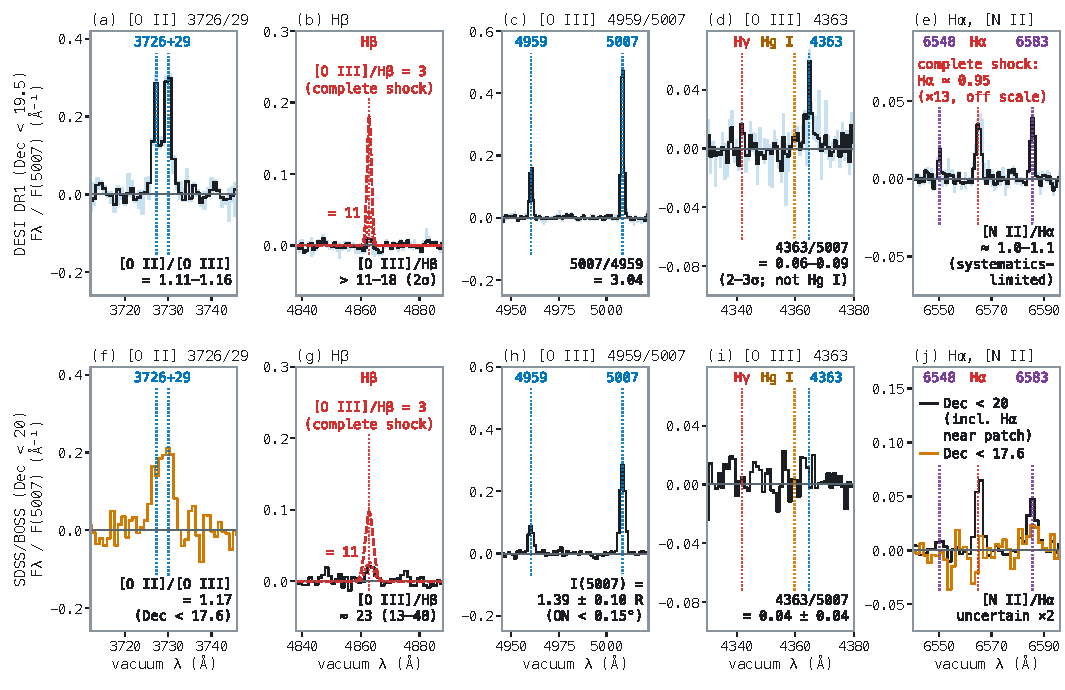
\includegraphics[width=\textwidth]{figures/w3_figs_f4_spectra.pdf}
\caption{Spectrum of the filament: flux density per \AA\ in units of the \Oiii~$\lambda5007$ flux (energy units) against vacuum wavelength. (a)--(e) DESI DR1 template regression \citep{DESI2026} for trace Dec $<19.5^{\circ}$; shading, 16--84\% HEALPix block-bootstrap range. (f)--(j) SDSS/BOSS total-sky ON$-$OFF stacks \citep{Abdurrouf2022} at Dec $<20^{\circ}$ (ON fibers within $0.15^{\circ}$ of a strand), except (f), seven BOSS groups at Dec $<17.6^{\circ}$ normalized to their own \Oiii~$\lambda5007$, and the Dec $<17.6^{\circ}$ curve in (j), which excludes \Ha\ structure near the \Ha\ patch. In (b) and (g), Gaussians at the \Oiii\ line width show \Oiii/\Hb\ $=3$ (dashed; complete shock) and 11 (dotted); (d) and (i) mark H$\gamma$ and \ion{Hg}{1}~$\lambda4358$; (e) notes the \Ha\ of a complete shock (0.95, off scale). Dotted vertical lines mark the lines at \vhel\ $=+13$\,\kms; annotations give measured values (Table~\ref{tab:ratios}).\label{fig:spectra}}
\end{figure*}

\subsection{Counterparts at other wavelengths and precovery}\label{sec:counterparts}

GALEX \citep{Martin2005,Morrissey2007} FUV and NUV images show a narrow ridge on the southern \Oiii\ spine (Figure~\ref{fig:profiles}b,c), at 68--92 (FUV; $8.7\sigma$ in a template regression on the \Oiii\ map) and 36--57\,CU (NUV) per rayleigh of \Oiii~$\lambda$5007 on the NSNS scale ($\approx85$--115 for the FUV on the DESI scale; no coverage north of Dec $+22^{\circ}$). Dust-scattered light contributes at most 34 (FUV) and 16\,CU (NUV), well below the measured ridge amplitudes of $172\pm32$ and $141\pm33$\,CU (Figure~\ref{fig:profiles}b,c).

No other tracer shows the filament (Figure~\ref{fig:profiles}d--g). In \Ha, SHASSA \citep{Gaustad2001}, the only arcminute-resolution survey of the spine (Dec 12--15.6$^{\circ}$), gives $<0.77$\,R, and WHAM \citep{Haffner2003} shows the same emission on and off the filament (Section~\ref{sec:shock}). GALFA-\ion{H}{1} \citep{Peek2018} shows no \ion{H}{1} filament, wall, cavity or velocity signature ($<1.0$--$1.75\times10^{19}$\,cm$^{-2}$ per 2\,\kms\ channel), IRIS 100\,$\mu$m \citep{MivilleDeschenes2005} no dust ($\Delta E(B-V)<0.004$), eRASS1 0.2--0.6\,keV \citep{Merloni2024} no X-ray filament, and the single-dish 408\,MHz survey \citep{Haslam1982} no total-intensity counterpart: $\Sigma_{\rm 1\,GHz}<1.3\times10^{-22}$\,W\,m$^{-2}$\,Hz$^{-1}$\,sr$^{-1}$ ($2\sigma$; corrected for beam dilution and extrapolated to 1\,GHz with $S_\nu\propto\nu^{-0.5}$).

A ridge template fitted to SDSS imaging sky levels \citep{Almeida2023} in 19 $g$-band runs from 2002--2007 gives $2.3\pm0.4$\,R ($3.9\sigma$ against coherent nulls; 1.4--4.6$\sigma$ across estimators), with no signal in $r$ or $i$, as expected for line emission; the earliest $\ge3\sigma$ run dates from 2002 December~31. SDSS sky fibers detect the filament from 2003 January~30 ($3.4\sigma$) and at $\ge5\sigma$ from 2005 March~3. Its brightness varied by less than a factor of $\approx2$ over 2002--2022. Digitized Sky Survey (DSS) plates do not detect it ($3\sigma$ limit $\approx40$\,R in DSS2 $J$).

\begin{figure*}
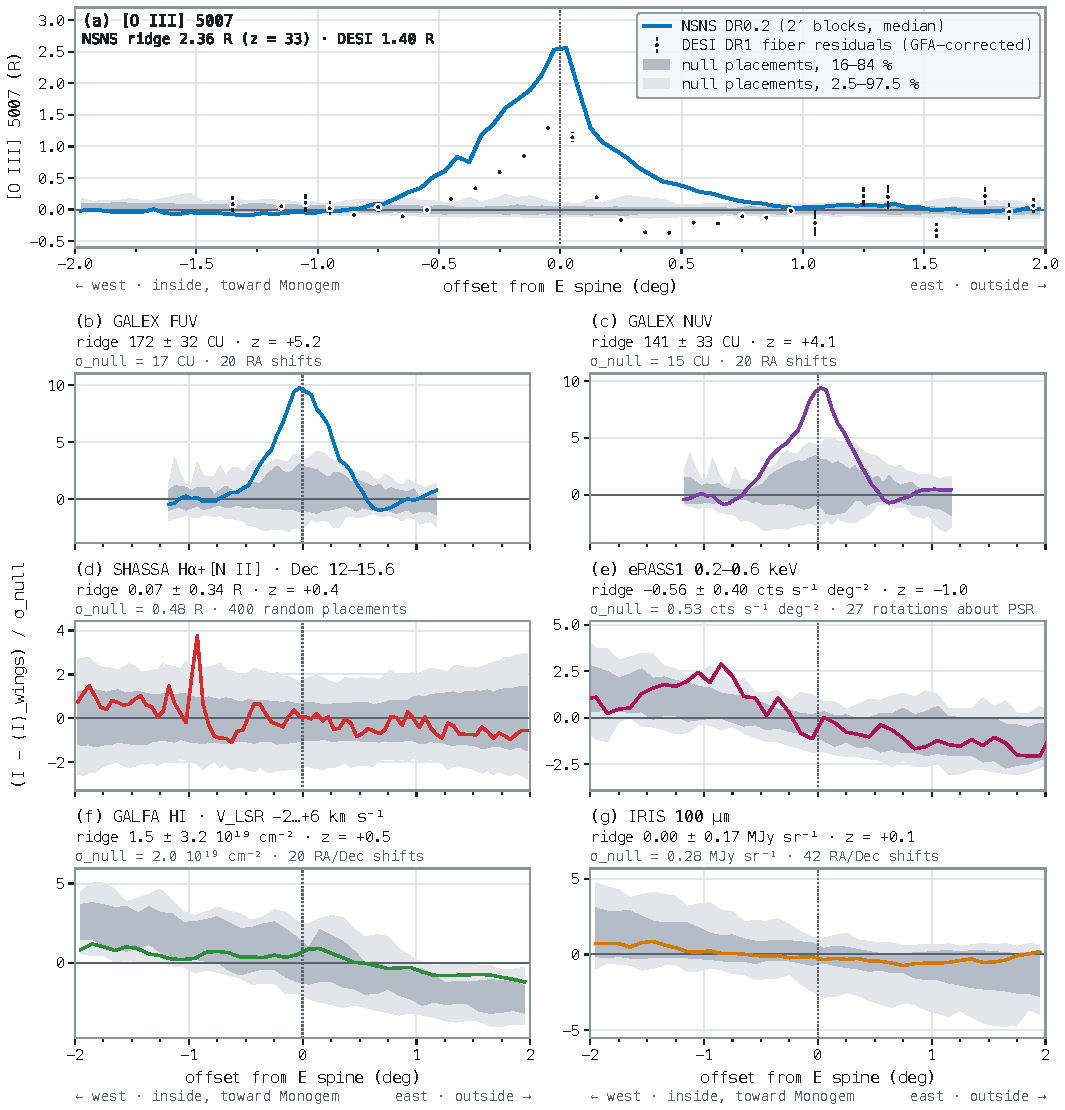
\includegraphics[width=\textwidth]{figures/w3_figs_f6_profiles.pdf}
\caption{Profiles across the southern spine (Dec $<17.6^{\circ}$) against offset $x$ from the E spine (positive eastward). (a) \Oiii~$\lambda$5007: NSNS DR0.2 map \citep[median in $2'$ blocks;][]{Ziegenbalg2025} and DESI DR1 fiber residuals \citep[mean $\pm$ s.e.;][]{DESI2026}, scaled by the guide-camera (GFA) fiber acceptance and relative to the per-petal sky mean, hence negative beside the ridge. (b, c) GALEX FUV and NUV \citep{Martin2005}; (d) SHASSA \Ha+\Nii\ \citep{Gaustad2001}; (e) eRASS1 \citep{Merloni2024}; (f) GALFA-\ion{H}{1} column density \citep{Peek2018}; (g) IRIS \citep{MivilleDeschenes2005}. In (b)--(g) each profile, minus its mean over the wings ($|x|\ge0.5^{\circ}$), is divided by $\sigma_{\rm null}$, the median per-bin scatter of null profiles (shifted or randomly placed traces; eRASS1: rotations about PSR B0656+14). Shading: 16--84\% and 2.5--97.5\% null ranges. Headers: fitted amplitude of a Gaussian ridge (FWHM $0.28^{\circ}$) $\pm$ the scatter of null amplitudes, and significance $z$.\label{fig:profiles}}
\end{figure*}

\subsection{Excitation mechanism}\label{sec:excitation}

We compared these constraints with plane-parallel non-equilibrium-ionization models of steady radiative shocks, complete or truncated at a swept-up column $N_*$ (no radiative transfer, so \Hb\ at intermediate columns is about half that of \citealt{Raymond1988} and each fit is repeated with model \Hb\ $\times2.3$; validated against \citealt{Raymond1979,Raymond1988,Allen2008,Gnat2007}; ultraviolet emissivities from CHIANTI v7.1, \citealt{Dere1997,Landi2013}), and with simplified models of the alternatives (Figure~\ref{fig:diagnostics}).

The spectrum rejects photoionization equilibrium at $p\le0.007$ ($\chi^2=21$--51 for 8 terms; $\chi^2=18$--25, $p\le0.02$, if $\lambda4363$ is floor-limited), which reaches only \Oiii/\Hb\ $\lesssim10$--14 and $\lambda4363/\lambda5007\lesssim0.012$--0.034 (diffuse ionized gas: \Oiii/\Hb\ $\le1.3$), and gives \ion{He}{2}/\Oiii\ $=0.06$ for a hot-gas ionizing spectrum (observed: $<0.026$). Even the most favorable cataloged ionizing source, the 81\,kK white dwarf WD~J0736+1444 \citep{Reindl2023}, gives an ionization parameter 18--30 times too low. Complete radiative shocks are excluded ($\chi^2\ge37$ for 10 terms): they reach only \Oiii/\Hb\ $\le5$ (published grids: 1.2--4.5; \citealt{Raymond1979,Cox1985,Dopita1996,Allen2008}), would produce an \Ha\ filament and cooled \ion{H}{1}, and their non-resonant ultraviolet lines alone (85--277\,CU per R) reach or exceed the measured FUV.

Turbulent mixing layers \citep{Slavin1993} and non-equilibrium cooling of the Monogem hot gas \citep{Gnat2007} can match the optical ratios but predict a soft X-ray filament $10^3$--$10^4$ times brighter than the Monogem shell, which eRASS1 excludes. Conduction fronts \citep{Borkowski1990} match them marginally but are excluded by their non-resonant FUV floor of 179--213\,CU per R, above the measured 68--92; they would also need $P/k\approx9\times10^5$\,K\,cm$^{-3}$ to be as narrow as the filament (1.4\,pc at 282\,pc; Section~\ref{sec:location}). A layer statically heated to $\approx6\times10^4$\,K fits the optical ratios ($\chi^2=6.2$ for 9 terms) but requires an unidentified, shock-sized heating flux ($0.5$--$2.6\times10^{-5}$\,erg\,cm$^{-2}$\,s$^{-1}$), and predicts \ion{C}{4}/\Oiii\ 4--10 times below the 0.15--0.4 (photons) implied by the FIMS/SPEAR map of \citet{Kim2007} if its region R1 (a $\approx2\sigma$ spatial match) is the Silk; it is disfavored but not excluded. Photoionization with extra heating to $4\times10^4$\,K also fits the optical ratios ($\chi^2=1.0$--2.4 for 9 terms) but needs 78--350 times the photoionization heating rate and the same missing ionizing source.

A column-truncated (incomplete) radiative shock \citep{Raymond1988} reproduces the line ratios ($\chi^2=0.3$ for 10 terms and four parameters, with 279 of the 480 grid models within $\Delta\chi^2=4$; Figure~\ref{fig:diagnostics}) and the FUV level, but overpredicts the NUV by a factor of 1.5--2 (79--99 against 36--57\,CU per R), comparable to the model systematic. In this model the post-shock gas radiates \Oiii\ and \Oii\ as it cools, but the flow ends before hydrogen recombines, leaving the Balmer lines weak. The optical ratios require $v_s\ge80$\,\kms\ and $\log N_*=17.4$--18.7 (cm$^{-2}$); the FUV level favors 80--120\,\kms\ ($\lesssim150$\,\kms). The acceptable models predict \Oiii/\Hb\ $=13$--62, \Oii/\Oiii\ $=1.0$--1.8 and $\lambda4363/\lambda5007=0.08$--0.10. The nearly symmetric southern cross-profile ($\sigma_W/\sigma_E=1.07$) favors an edge-on flat or gently curved sheet over a smooth curved limb ($\approx2\sigma$). For such a sheet at 282\,pc the models give $P/k\approx1.2\times10^4$--$5.5\times10^5$\,K\,cm$^{-3}$ and a pre-shock density $n_0\approx0.012$--0.13\,cm$^{-3}$ (both $\propto d^{-1}$), the latter $\sim$35--370 times lower than in the Cygnus Loop filaments of \citet{Raymond1988}; resonance scattering of \ion{C}{4} within the sheet brings the predicted FUV to 68--143\,CU per R.

Two tensions remain. DESI places the \Oii\ ridge 0.04--0.05$^{\circ}$ east of the \Oiii\ ridge, whereas a plane shock places it downstream, to the west (disfavored at $p\approx0.003$--0.07). The DESI \Oii~$\lambda3729/\lambda3726$ ratio (Table~\ref{tab:ratios}) lies 2.1--2.7$\sigma$ below the low-density limit that every scenario predicts.

\begin{figure*}
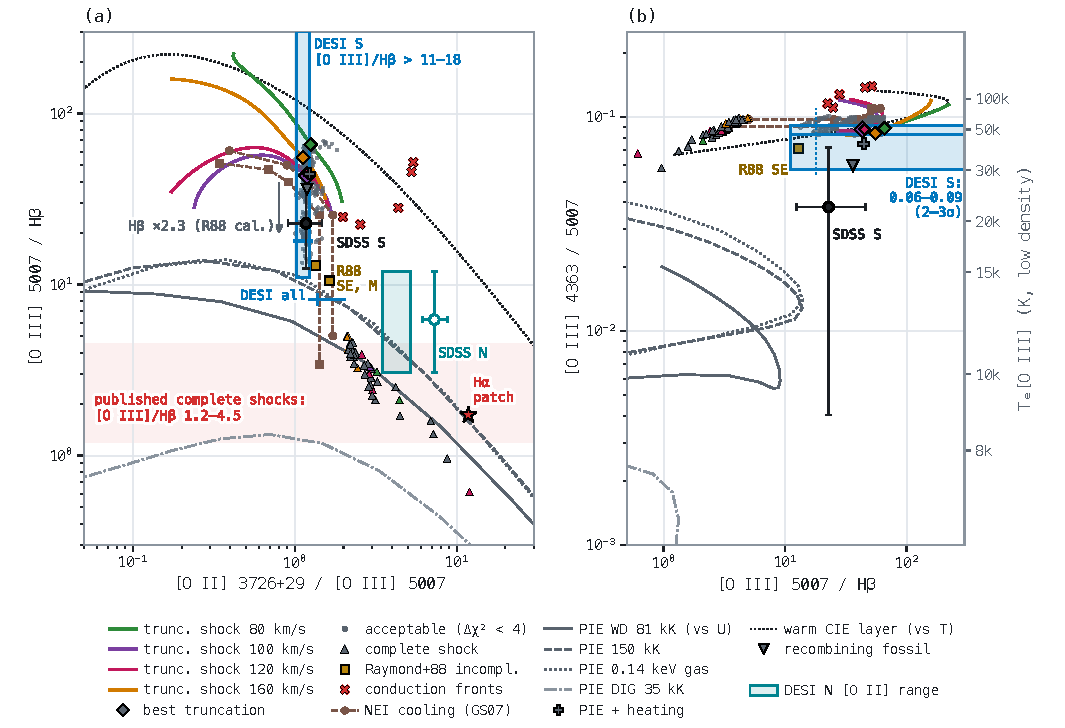
\includegraphics[width=\textwidth]{figures/w3_figs_f5_diagnostics.pdf}
\caption{Observed line ratios (energy units) and model loci. (a) \Oiii~$\lambda5007$/\Hb\ against \Oii~$\lambda\lambda3726,3729$/\Oiii~$\lambda5007$. (b) \Oiii~$\lambda4363/\lambda5007$ (right axis: low-density $T_e$) against \Oiii~$\lambda5007$/\Hb. S, N: southern, northern filament. DESI~S boxes start at the $2\sigma$ limit \Oiii/\Hb\ $>11$; the tick in (a) and the dotted line in (b) mark the Gaussian-fit limit, 18. SDSS~S combines \Oii/\Oiii\ at Dec $<17.6^{\circ}$ (95\% bar) with \Oiii/\Hb\ at Dec $<20^{\circ}$ (68\% bar). `DESI all' has an arbitrary ordinate; the DESI~N \Oii/\Oiii\ range is drawn over the SDSS~N \Oiii/\Hb\ range. Truncated-shock (trunc.) tracks: cumulative ratios against swept-up column for the best run at each $v_s$; diamonds, best truncations; dots, all runs within $\Delta\chi^2<4$. R88: incomplete-shock models SE and M of \citet{Raymond1988}. PIE: photoionization equilibrium against ionization parameter $U$ (kK: blackbody temperature; WD: WD~J0736+1444; DIG: diffuse ionized gas); plus sign, PIE with extra heating to $4\times10^4$\,K. Inverted triangle: unheated gas recombining from $4\times10^4$\,K. NEI: non-equilibrium cooling of hot gas \citep[GS07;][]{Gnat2007}, isobaric (circles) and isochoric (squares). CIE: collisional ionization equilibrium. Arrow: model \Hb\ $\times2.3$ (R88 calibration). Star in (a): the \Ha\ patch (SDSS; Section~\ref{sec:spectrum}). Shading in (a): published complete shocks \citep{Raymond1979,Cox1985,Dopita1996,Allen2008}.\label{fig:diagnostics}}
\end{figure*}

\subsection{Location and distance}\label{sec:location}

An edge-on shock moves in the plane of the sky, so its line-of-sight velocity is that of the pre-shock gas. The \Oiii\ shares the velocity of the local WIM and \ion{H}{1} (\vlsr\ $\approx0$--2\,\kms); the northern redshift matches a northern \ion{H}{1} component at \vlsr\ $=+8.5$ to $+11.3$\,\kms, possibly the pre-shock gas.

The southern spine (Dec $<17.6^{\circ}$) lies $12.10\pm0.12^{\circ}$ from the two-remnant center of \citet{Knies2024}, close to their Monogem shell radius ($11.0\pm1.1^{\circ}$), and follows the outer half-maximum contour of the eRASS1 0.2--0.6\,keV emission in its position-angle sector for every proposed center (offsets $-0.06\pm0.14^{\circ}$ to $+0.19\pm0.09^{\circ}$; $p\approx0.03$--0.05 against rotations). A rigid trace placed at random in the same latitude band and reaching the rim matches the shell radius about any of three proposed centers with probability 0.09. These coincidences favor, but do not establish, a location on the Monogem limb, which lies at 252--318\,pc (68\%; median 282\,pc) if the shell is centered at the parallax distance of PSR B0656+14 ($288^{+33}_{-27}$\,pc; \citealt{Brisken2003}). The southern spine is straighter than this circle (radius of curvature $\approx67^{\circ}$) and only tangent to it; north of Dec $+18.5^{\circ}$ the arc leaves it.

Two further tests do not strengthen the association. Stellar extinctions \citep{Anders2022,Gaia2023} suggest that the cold clump PGCC G199.09+19.95 \citep{Planck2016}, which adjoins the \Ha\ patch on the same circle, lies beyond the limb, at $\approx400$--650\,pc (2--2.5$\sigma$; catalog value $262\pm121$\,pc). E1, a fainter \Oiii\ filament farther east \citep{Fesen2026}, has a similar Balmer-faint DESI spectrum but \vlsr\ $=-24\pm2.5$\,\kms, so the eastern Monogem filaments do not share one velocity.

No measurement fixes the distance: the velocity carries no distance information (Section~\ref{sec:distance}), no absorption line brackets the ionized gas, and no dust is detected. Distances of $\sim$100\,pc to $\sim$1\,kpc are allowed, including the 160\,pc adopted by W26. The $\approx1.6$\,kpc implied by W26 Table~4 is disfavored: the filament would be $\approx470$\,pc long at a height $z\approx0.55$\,kpc above the Galactic plane, with a north--south velocity gradient opposite in sign to Galactic rotation.
